\documentclass[1p]{elsarticle_modified}
%\bibliographystyle{elsarticle-num}

%\usepackage[colorlinks]{hyperref}
%\usepackage{abbrmath_seonhwa} %\Abb, \Ascr, \Acal ,\Abf, \Afrak
\usepackage{amsfonts}
\usepackage{amssymb}
\usepackage{amsmath}
\usepackage{amsthm}
\usepackage{scalefnt}
\usepackage{amsbsy}
\usepackage{kotex}
\usepackage{caption}
\usepackage{subfig}
\usepackage{color}
\usepackage{graphicx}
\usepackage{xcolor} %% white, black, red, green, blue, cyan, magenta, yellow
\usepackage{float}
\usepackage{setspace}
\usepackage{hyperref}

\usepackage{tikz}
\usetikzlibrary{arrows}

\usepackage{multirow}
\usepackage{array} % fixed length table
\usepackage{hhline}

%%%%%%%%%%%%%%%%%%%%%
\makeatletter
\renewcommand*\env@matrix[1][\arraystretch]{%
	\edef\arraystretch{#1}%
	\hskip -\arraycolsep
	\let\@ifnextchar\new@ifnextchar
	\array{*\c@MaxMatrixCols c}}
\makeatother %https://tex.stackexchange.com/questions/14071/how-can-i-increase-the-line-spacing-in-a-matrix
%%%%%%%%%%%%%%%

\usepackage[normalem]{ulem}

\newcommand{\msout}[1]{\ifmmode\text{\sout{\ensuremath{#1}}}\else\sout{#1}\fi}
%SOURCE: \msout is \stkout macro in https://tex.stackexchange.com/questions/20609/strikeout-in-math-mode

\newcommand{\cancel}[1]{
	\ifmmode
	{\color{red}\msout{#1}}
	\else
	{\color{red}\sout{#1}}
	\fi
}

\newcommand{\add}[1]{
	{\color{blue}\uwave{#1}}
}

\newcommand{\replace}[2]{
	\ifmmode
	{\color{red}\msout{#1}}{\color{blue}\uwave{#2}}
	\else
	{\color{red}\sout{#1}}{\color{blue}\uwave{#2}}
	\fi
}

\newcommand{\Sol}{\mathcal{S}} %segment
\newcommand{\D}{D} %diagram
\newcommand{\A}{\mathcal{A}} %arc


%%%%%%%%%%%%%%%%%%%%%%%%%%%%%5 test

\def\sl{\operatorname{\textup{SL}}(2,\Cbb)}
\def\psl{\operatorname{\textup{PSL}}(2,\Cbb)}
\def\quan{\mkern 1mu \triangleright \mkern 1mu}

\theoremstyle{definition}
\newtheorem{thm}{Theorem}[section]
\newtheorem{prop}[thm]{Proposition}
\newtheorem{lem}[thm]{Lemma}
\newtheorem{ques}[thm]{Question}
\newtheorem{cor}[thm]{Corollary}
\newtheorem{defn}[thm]{Definition}
\newtheorem{exam}[thm]{Example}
\newtheorem{rmk}[thm]{Remark}
\newtheorem{alg}[thm]{Algorithm}

\newcommand{\I}{\sqrt{-1}}
\begin{document}

%\begin{frontmatter}
%
%\title{Boundary parabolic representations of knots up to 8 crossings}
%
%%% Group authors per affiliation:
%\author{Yunhi Cho} 
%\address{Department of Mathematics, University of Seoul, Seoul, Korea}
%\ead{yhcho@uos.ac.kr}
%
%
%\author{Seonhwa Kim} %\fnref{s_kim}}
%\address{Center for Geometry and Physics, Institute for Basic Science, Pohang, 37673, Korea}
%\ead{ryeona17@ibs.re.kr}
%
%\author{Hyuk Kim}
%\address{Department of Mathematical Sciences, Seoul National University, Seoul 08826, Korea}
%\ead{hyukkim@snu.ac.kr}
%
%\author{Seokbeom Yoon}
%\address{Department of Mathematical Sciences, Seoul National University, Seoul, 08826,  Korea}
%\ead{sbyoon15@snu.ac.kr}
%
%\begin{abstract}
%We find all boundary parabolic representation of knots up to 8 crossings.
%
%\end{abstract}
%\begin{keyword}
%    \MSC[2010] 57M25 
%\end{keyword}
%
%\end{frontmatter}

%\linenumbers
%\tableofcontents
%
\newcommand\colored[1]{\textcolor{white}{\rule[-0.35ex]{0.8em}{1.4ex}}\kern-0.8em\color{red} #1}%
%\newcommand\colored[1]{\textcolor{white}{ #1}\kern-2.17ex	\textcolor{white}{ #1}\kern-1.81ex	\textcolor{white}{ #1}\kern-2.15ex\color{red}#1	}

{\Large $\underline{11a_{97}~(K11a_{97})}$}

\setlength{\tabcolsep}{10pt}
\renewcommand{\arraystretch}{1.6}
\vspace{1cm}\begin{tabular}{m{100pt}>{\centering\arraybackslash}m{274pt}}
\multirow{5}{120pt}{
	\centering
	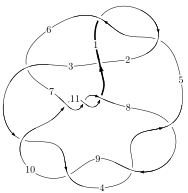
\includegraphics[width=112pt]{../../../GIT/diagram.site/Diagrams/png/346_11a_97.png}\\
\ \ \ A knot diagram\footnotemark}&
\allowdisplaybreaks
\textbf{Linearized knot diagam} \\
\cline{2-2}
 &
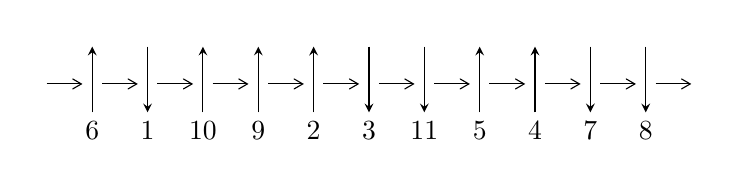
\begin{tikzpicture}[x=20pt, y=17pt]
	% nodes
	\node (C0) at (0, 0) {};
	\node (C1) at (1, 0) {};
	\node (C1U) at (1, +1) {};
	\node (C1D) at (1, -1) {6};

	\node (C2) at (2, 0) {};
	\node (C2U) at (2, +1) {};
	\node (C2D) at (2, -1) {1};

	\node (C3) at (3, 0) {};
	\node (C3U) at (3, +1) {};
	\node (C3D) at (3, -1) {10};

	\node (C4) at (4, 0) {};
	\node (C4U) at (4, +1) {};
	\node (C4D) at (4, -1) {9};

	\node (C5) at (5, 0) {};
	\node (C5U) at (5, +1) {};
	\node (C5D) at (5, -1) {2};

	\node (C6) at (6, 0) {};
	\node (C6U) at (6, +1) {};
	\node (C6D) at (6, -1) {3};

	\node (C7) at (7, 0) {};
	\node (C7U) at (7, +1) {};
	\node (C7D) at (7, -1) {11};

	\node (C8) at (8, 0) {};
	\node (C8U) at (8, +1) {};
	\node (C8D) at (8, -1) {5};

	\node (C9) at (9, 0) {};
	\node (C9U) at (9, +1) {};
	\node (C9D) at (9, -1) {4};

	\node (C10) at (10, 0) {};
	\node (C10U) at (10, +1) {};
	\node (C10D) at (10, -1) {7};

	\node (C11) at (11, 0) {};
	\node (C11U) at (11, +1) {};
	\node (C11D) at (11, -1) {8};
	\node (C12) at (12, 0) {};

	% arrows
	\draw[->,>={angle 60}]
	(C0) edge (C1) (C1) edge (C2) (C2) edge (C3) (C3) edge (C4) (C4) edge (C5) (C5) edge (C6) (C6) edge (C7) (C7) edge (C8) (C8) edge (C9) (C9) edge (C10) (C10) edge (C11) (C11) edge (C12) ;	\draw[->,>=stealth]
	(C1D) edge (C1U) (C2U) edge (C2D) (C3D) edge (C3U) (C4D) edge (C4U) (C5D) edge (C5U) (C6U) edge (C6D) (C7U) edge (C7D) (C8D) edge (C8U) (C9D) edge (C9U) (C10U) edge (C10D) (C11U) edge (C11D) ;
	\end{tikzpicture} \\
\hhline{~~} \\& 
\textbf{Solving Sequence} \\ \cline{2-2} 
 &
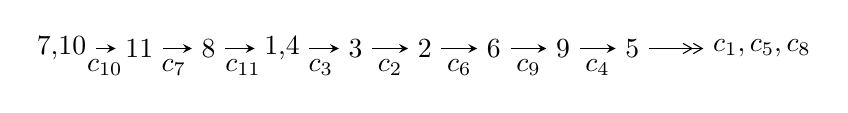
\begin{tikzpicture}[x=25pt, y=7pt]
	% node
	\node (A0) at (-1/8, 0) {7,10};
	\node (A1) at (1, 0) {11};
	\node (A2) at (2, 0) {8};
	\node (A3) at (49/16, 0) {1,4};
	\node (A4) at (33/8, 0) {3};
	\node (A5) at (41/8, 0) {2};
	\node (A6) at (49/8, 0) {6};
	\node (A7) at (57/8, 0) {9};
	\node (A8) at (65/8, 0) {5};
	\node (C1) at (1/2, -1) {$c_{10}$};
	\node (C2) at (3/2, -1) {$c_{7}$};
	\node (C3) at (5/2, -1) {$c_{11}$};
	\node (C4) at (29/8, -1) {$c_{3}$};
	\node (C5) at (37/8, -1) {$c_{2}$};
	\node (C6) at (45/8, -1) {$c_{6}$};
	\node (C7) at (53/8, -1) {$c_{9}$};
	\node (C8) at (61/8, -1) {$c_{4}$};
	\node (A9) at (10, 0) {$c_{1},c_{5},c_{8}$};

	% edge
	\draw[->,>=stealth]	
	(A0) edge (A1) (A1) edge (A2) (A2) edge (A3) (A3) edge (A4) (A4) edge (A5) (A5) edge (A6) (A6) edge (A7) (A7) edge (A8) ;
	\draw[->>,>={angle 60}]	
	(A8) edge (A9);
\end{tikzpicture} \\ 

\end{tabular} \\

\footnotetext{
The image of knot diagram is generated by the software ``\textbf{Draw programme}" developed by Andrew Bartholomew(\url{http://www.layer8.co.uk/maths/draw/index.htm\#Running-draw}), where we modified some parts for our purpose(\url{https://github.com/CATsTAILs/LinksPainter}).
}\phantom \\ \newline 
\centering \textbf{Ideals for irreducible components\footnotemark of $X_{\text{par}}$} 
 
\begin{align*}
I^u_{1}&=\langle 
1.35647\times10^{26} u^{40}+3.41407\times10^{25} u^{39}+\cdots+4.76775\times10^{26} b+1.22986\times10^{27},\\
\phantom{I^u_{1}}&\phantom{= \langle  }1.32011\times10^{27} u^{40}-3.91635\times10^{27} u^{39}+\cdots+5.72130\times10^{27} a+9.91592\times10^{27},\;u^{41}+3 u^{40}+\cdots-16 u+3\rangle \\
I^u_{2}&=\langle 
-2 a^3-3 a^2+5 b-15 a-7,\;a^4+2 a^3+7 a^2+6 a+3,\;u-1\rangle \\
I^u_{3}&=\langle 
b,\;a^2+a+1,\;u+1\rangle \\
\\
\end{align*}
\raggedright * 3 irreducible components of $\dim_{\mathbb{C}}=0$, with total 47 representations.\\
\footnotetext{All coefficients of polynomials are rational numbers. But the coefficients are sometimes approximated in decimal forms when there is not enough margin.}
\newpage
\renewcommand{\arraystretch}{1}
\centering \section*{I. $I^u_{1}= \langle 1.36\times10^{26} u^{40}+3.41\times10^{25} u^{39}+\cdots+4.77\times10^{26} b+1.23\times10^{27},\;1.32\times10^{27} u^{40}-3.92\times10^{27} u^{39}+\cdots+5.72\times10^{27} a+9.92\times10^{27},\;u^{41}+3 u^{40}+\cdots-16 u+3 \rangle$}
\flushleft \textbf{(i) Arc colorings}\\
\begin{tabular}{m{7pt} m{180pt} m{7pt} m{180pt} }
\flushright $a_{7}=$&$\begin{pmatrix}0\\u\end{pmatrix}$ \\
\flushright $a_{10}=$&$\begin{pmatrix}1\\0\end{pmatrix}$ \\
\flushright $a_{11}=$&$\begin{pmatrix}1\\u^2\end{pmatrix}$ \\
\flushright $a_{8}=$&$\begin{pmatrix}- u\\- u^3+u\end{pmatrix}$ \\
\flushright $a_{1}=$&$\begin{pmatrix}- u^2+1\\- u^4+2 u^2\end{pmatrix}$ \\
\flushright $a_{4}=$&$\begin{pmatrix}-0.230736 u^{40}+0.684521 u^{39}+\cdots+27.5823 u-1.73316\\-0.284509 u^{40}-0.0716075 u^{39}+\cdots+13.5631 u-2.57954\end{pmatrix}$ \\
\flushright $a_{3}=$&$\begin{pmatrix}0.0537729 u^{40}+0.756128 u^{39}+\cdots+14.0192 u+0.846378\\-0.284509 u^{40}-0.0716075 u^{39}+\cdots+13.5631 u-2.57954\end{pmatrix}$ \\
\flushright $a_{2}=$&$\begin{pmatrix}-0.417033 u^{40}+0.180050 u^{39}+\cdots+24.6975 u-0.635993\\-0.488200 u^{40}-0.376850 u^{39}+\cdots+16.4598 u-3.17299\end{pmatrix}$ \\
\flushright $a_{6}=$&$\begin{pmatrix}-0.699060 u^{40}-0.274328 u^{39}+\cdots+36.6179 u-7.70938\\-0.662144 u^{40}-0.883819 u^{39}+\cdots+14.3253 u-3.84461\end{pmatrix}$ \\
\flushright $a_{9}=$&$\begin{pmatrix}2.14850 u^{40}+4.44463 u^{39}+\cdots+10.3774 u-6.62221\\0.866962 u^{40}+1.26216 u^{39}+\cdots-10.7057 u-0.442876\end{pmatrix}$ \\
\flushright $a_{5}=$&$\begin{pmatrix}0.516885 u^{40}+0.0710561 u^{39}+\cdots-22.2661 u+0.886590\\0.526631 u^{40}+0.306983 u^{39}+\cdots-19.7993 u+3.74658\end{pmatrix}$\\ \flushright $a_{5}=$&$\begin{pmatrix}0.516885 u^{40}+0.0710561 u^{39}+\cdots-22.2661 u+0.886590\\0.526631 u^{40}+0.306983 u^{39}+\cdots-19.7993 u+3.74658\end{pmatrix}$\\&\end{tabular}
\flushleft \textbf{(ii) Obstruction class $= -1$}\\~\\
\flushleft \textbf{(iii) Cusp Shapes $= \frac{559898241088593396717061691}{238387645942441547003348479} u^{40}+\frac{403977182003809318732241725}{86686416706342380728490356} u^{39}+\cdots-\frac{465164699436934167876296904}{238387645942441547003348479} u+\frac{633526497906639455712438183}{953550583769766188013393916}$}\\~\\
\newpage\renewcommand{\arraystretch}{1}
\flushleft \textbf{(iv) u-Polynomials at the component}\newline \\
\begin{tabular}{m{50pt}|m{274pt}}
Crossings & \hspace{64pt}u-Polynomials at each crossing \\
\hline $$\begin{aligned}c_{1},c_{5}\end{aligned}$$&$\begin{aligned}
&u^{41}-2 u^{40}+\cdots+3 u-3
\end{aligned}$\\
\hline $$\begin{aligned}c_{2}\end{aligned}$$&$\begin{aligned}
&u^{41}+22 u^{40}+\cdots-33 u-9
\end{aligned}$\\
\hline $$\begin{aligned}c_{3},c_{4},c_{8}\\c_{9}\end{aligned}$$&$\begin{aligned}
&u^{41}- u^{40}+\cdots+8 u+4
\end{aligned}$\\
\hline $$\begin{aligned}c_{6}\end{aligned}$$&$\begin{aligned}
&u^{41}+2 u^{40}+\cdots+327 u-87
\end{aligned}$\\
\hline $$\begin{aligned}c_{7},c_{10},c_{11}\end{aligned}$$&$\begin{aligned}
&u^{41}+3 u^{40}+\cdots-16 u+3
\end{aligned}$\\
\hline
\end{tabular}\\~\\
\newpage\renewcommand{\arraystretch}{1}
\flushleft \textbf{(v) Riley Polynomials at the component}\newline \\
\begin{tabular}{m{50pt}|m{274pt}}
Crossings & \hspace{64pt}Riley Polynomials at each crossing \\
\hline $$\begin{aligned}c_{1},c_{5}\end{aligned}$$&$\begin{aligned}
&y^{41}+22 y^{40}+\cdots-33 y-9
\end{aligned}$\\
\hline $$\begin{aligned}c_{2}\end{aligned}$$&$\begin{aligned}
&y^{41}-2 y^{40}+\cdots+423 y-81
\end{aligned}$\\
\hline $$\begin{aligned}c_{3},c_{4},c_{8}\\c_{9}\end{aligned}$$&$\begin{aligned}
&y^{41}+51 y^{40}+\cdots-128 y-16
\end{aligned}$\\
\hline $$\begin{aligned}c_{6}\end{aligned}$$&$\begin{aligned}
&y^{41}-26 y^{40}+\cdots-166425 y-7569
\end{aligned}$\\
\hline $$\begin{aligned}c_{7},c_{10},c_{11}\end{aligned}$$&$\begin{aligned}
&y^{41}-43 y^{40}+\cdots+4 y-9
\end{aligned}$\\
\hline
\end{tabular}\\~\\
\newpage\flushleft \textbf{(vi) Complex Volumes and Cusp Shapes}
$$\begin{array}{c|c|c}  
\text{Solutions to }I^u_{1}& \I (\text{vol} + \sqrt{-1}CS) & \text{Cusp shape}\\
 \hline 
\begin{aligned}
u &= -0.997009 + 0.226554 I \\
a &= \phantom{-}0.0239968 + 0.0485183 I \\
b &= \phantom{-}0.302628 - 0.382168 I\end{aligned}
 & -2.03507 + 1.22420 I & -5.30574 + 2.47978 I \\ \hline\begin{aligned}
u &= -0.997009 - 0.226554 I \\
a &= \phantom{-}0.0239968 - 0.0485183 I \\
b &= \phantom{-}0.302628 + 0.382168 I\end{aligned}
 & -2.03507 - 1.22420 I & -5.30574 - 2.47978 I \\ \hline\begin{aligned}
u &= \phantom{-}0.549974 + 0.797423 I \\
a &= \phantom{-}0.960310 + 0.778214 I \\
b &= -0.05763 + 1.60436 I\end{aligned}
 & -7.81669 - 2.63616 I & -2.57791 + 2.58719 I \\ \hline\begin{aligned}
u &= \phantom{-}0.549974 - 0.797423 I \\
a &= \phantom{-}0.960310 - 0.778214 I \\
b &= -0.05763 - 1.60436 I\end{aligned}
 & -7.81669 + 2.63616 I & -2.57791 - 2.58719 I \\ \hline\begin{aligned}
u &= \phantom{-}0.507571 + 0.956182 I \\
a &= -0.888380 - 0.590788 I \\
b &= \phantom{-}0.09789 - 1.64453 I\end{aligned}
 & -10.92990 - 7.37639 I & -5.80773 + 5.55165 I \\ \hline\begin{aligned}
u &= \phantom{-}0.507571 - 0.956182 I \\
a &= -0.888380 + 0.590788 I \\
b &= \phantom{-}0.09789 + 1.64453 I\end{aligned}
 & -10.92990 + 7.37639 I & -5.80773 - 5.55165 I \\ \hline\begin{aligned}
u &= \phantom{-}0.762467 + 0.844946 I \\
a &= -0.710291 - 0.815437 I \\
b &= -0.00225 - 1.64871 I\end{aligned}
 & -11.70310 + 1.34196 I & -7.30625 - 0.70220 I \\ \hline\begin{aligned}
u &= \phantom{-}0.762467 - 0.844946 I \\
a &= -0.710291 + 0.815437 I \\
b &= -0.00225 + 1.64871 I\end{aligned}
 & -11.70310 - 1.34196 I & -7.30625 + 0.70220 I \\ \hline\begin{aligned}
u &= \phantom{-}1.137860 + 0.247744 I \\
a &= \phantom{-}0.169104 + 1.219170 I \\
b &= \phantom{-}0.12340 + 1.41903 I\end{aligned}
 & -7.87303 + 0.41748 I & -9.30153 + 0.50767 I \\ \hline\begin{aligned}
u &= \phantom{-}1.137860 - 0.247744 I \\
a &= \phantom{-}0.169104 - 1.219170 I \\
b &= \phantom{-}0.12340 - 1.41903 I\end{aligned}
 & -7.87303 - 0.41748 I & -9.30153 - 0.50767 I\\
 \hline 
 \end{array}$$\newpage$$\begin{array}{c|c|c}  
\text{Solutions to }I^u_{1}& \I (\text{vol} + \sqrt{-1}CS) & \text{Cusp shape}\\
 \hline 
\begin{aligned}
u &= -0.455355 + 0.700282 I \\
a &= -0.905605 - 0.022977 I \\
b &= \phantom{-}0.366148 + 0.772313 I\end{aligned}
 & -2.54750 + 5.63680 I & -3.76761 - 8.15870 I \\ \hline\begin{aligned}
u &= -0.455355 - 0.700282 I \\
a &= -0.905605 + 0.022977 I \\
b &= \phantom{-}0.366148 - 0.772313 I\end{aligned}
 & -2.54750 - 5.63680 I & -3.76761 + 8.15870 I \\ \hline\begin{aligned}
u &= -0.631099 + 0.496871 I \\
a &= -0.486895 - 0.221432 I \\
b &= \phantom{-}0.021123 + 0.779816 I\end{aligned}
 & -3.17977 - 1.35362 I & -6.58078 + 0.48937 I \\ \hline\begin{aligned}
u &= -0.631099 - 0.496871 I \\
a &= -0.486895 + 0.221432 I \\
b &= \phantom{-}0.021123 - 0.779816 I\end{aligned}
 & -3.17977 + 1.35362 I & -6.58078 - 0.48937 I \\ \hline\begin{aligned}
u &= \phantom{-}1.247250 + 0.042571 I \\
a &= -0.20681 - 1.71804 I \\
b &= \phantom{-}0.102712 - 0.658984 I\end{aligned}
 & -2.68106 - 2.54195 I & -5.78064 + 4.47516 I \\ \hline\begin{aligned}
u &= \phantom{-}1.247250 - 0.042571 I \\
a &= -0.20681 + 1.71804 I \\
b &= \phantom{-}0.102712 + 0.658984 I\end{aligned}
 & -2.68106 + 2.54195 I & -5.78064 - 4.47516 I \\ \hline\begin{aligned}
u &= -0.337954 + 0.540347 I \\
a &= \phantom{-}0.817560 - 0.128808 I \\
b &= -0.294187 - 0.599361 I\end{aligned}
 & -0.16445 + 1.48990 I & \phantom{-}0.43975 - 5.27239 I \\ \hline\begin{aligned}
u &= -0.337954 - 0.540347 I \\
a &= \phantom{-}0.817560 + 0.128808 I \\
b &= -0.294187 + 0.599361 I\end{aligned}
 & -0.16445 - 1.48990 I & \phantom{-}0.43975 + 5.27239 I \\ \hline\begin{aligned}
u &= -1.38121\phantom{ +0.000000I} \\
a &= -0.0677912\phantom{ +0.000000I} \\
b &= \phantom{-}0.707999\phantom{ +0.000000I}\end{aligned}
 & -3.43392\phantom{ +0.000000I} & \phantom{-0.000000 } 0 \\ \hline\begin{aligned}
u &= \phantom{-}1.45521 + 0.17025 I \\
a &= -0.414019 - 1.121630 I \\
b &= \phantom{-}0.508690 - 0.861076 I\end{aligned}
 & -6.01336 - 4.06181 I & \phantom{-0.000000 } 0\\
 \hline 
 \end{array}$$\newpage$$\begin{array}{c|c|c}  
\text{Solutions to }I^u_{1}& \I (\text{vol} + \sqrt{-1}CS) & \text{Cusp shape}\\
 \hline 
\begin{aligned}
u &= \phantom{-}1.45521 - 0.17025 I \\
a &= -0.414019 + 1.121630 I \\
b &= \phantom{-}0.508690 + 0.861076 I\end{aligned}
 & -6.01336 + 4.06181 I & \phantom{-0.000000 } 0 \\ \hline\begin{aligned}
u &= -1.47695 + 0.04519 I \\
a &= -0.26335 + 2.90182 I \\
b &= \phantom{-}0.02320 + 1.62981 I\end{aligned}
 & -10.76740 + 2.97655 I & \phantom{-0.000000 } 0 \\ \hline\begin{aligned}
u &= -1.47695 - 0.04519 I \\
a &= -0.26335 - 2.90182 I \\
b &= \phantom{-}0.02320 - 1.62981 I\end{aligned}
 & -10.76740 - 2.97655 I & \phantom{-0.000000 } 0 \\ \hline\begin{aligned}
u &= -1.48592 + 0.10113 I \\
a &= \phantom{-}0.0860114 - 0.0153300 I \\
b &= -0.823123 + 0.103447 I\end{aligned}
 & -6.74821 + 4.23995 I & \phantom{-0.000000 } 0 \\ \hline\begin{aligned}
u &= -1.48592 - 0.10113 I \\
a &= \phantom{-}0.0860114 + 0.0153300 I \\
b &= -0.823123 - 0.103447 I\end{aligned}
 & -6.74821 - 4.23995 I & \phantom{-0.000000 } 0 \\ \hline\begin{aligned}
u &= \phantom{-}0.385648 + 0.302544 I \\
a &= -1.59375 - 0.01228 I \\
b &= \phantom{-}0.456373 + 0.089106 I\end{aligned}
 & -0.52713 - 2.73009 I & \phantom{-}3.23724 + 4.11462 I \\ \hline\begin{aligned}
u &= \phantom{-}0.385648 - 0.302544 I \\
a &= -1.59375 + 0.01228 I \\
b &= \phantom{-}0.456373 - 0.089106 I\end{aligned}
 & -0.52713 + 2.73009 I & \phantom{-}3.23724 - 4.11462 I \\ \hline\begin{aligned}
u &= \phantom{-}1.52169 + 0.06207 I \\
a &= \phantom{-}0.267867 + 1.067660 I \\
b &= -0.490449 + 1.028460 I\end{aligned}
 & -10.25760 - 0.21541 I & \phantom{-0.000000 } 0 \\ \hline\begin{aligned}
u &= \phantom{-}1.52169 - 0.06207 I \\
a &= \phantom{-}0.267867 - 1.067660 I \\
b &= -0.490449 - 1.028460 I\end{aligned}
 & -10.25760 + 0.21541 I & \phantom{-0.000000 } 0 \\ \hline\begin{aligned}
u &= \phantom{-}1.51624 + 0.23392 I \\
a &= \phantom{-}0.450012 + 1.020390 I \\
b &= -0.618443 + 0.860508 I\end{aligned}
 & -9.03060 - 9.03490 I & \phantom{-0.000000 } 0\\
 \hline 
 \end{array}$$\newpage$$\begin{array}{c|c|c}  
\text{Solutions to }I^u_{1}& \I (\text{vol} + \sqrt{-1}CS) & \text{Cusp shape}\\
 \hline 
\begin{aligned}
u &= \phantom{-}1.51624 - 0.23392 I \\
a &= \phantom{-}0.450012 - 1.020390 I \\
b &= -0.618443 - 0.860508 I\end{aligned}
 & -9.03060 + 9.03490 I & \phantom{-0.000000 } 0 \\ \hline\begin{aligned}
u &= \phantom{-}0.046246 + 0.427515 I \\
a &= \phantom{-}1.224630 - 0.289199 I \\
b &= -0.391553 - 0.302388 I\end{aligned}
 & \phantom{-}0.667792 + 1.033690 I & \phantom{-}4.88372 - 5.04725 I \\ \hline\begin{aligned}
u &= \phantom{-}0.046246 - 0.427515 I \\
a &= \phantom{-}1.224630 + 0.289199 I \\
b &= -0.391553 + 0.302388 I\end{aligned}
 & \phantom{-}0.667792 - 1.033690 I & \phantom{-}4.88372 + 5.04725 I \\ \hline\begin{aligned}
u &= -1.55585 + 0.27915 I \\
a &= -0.94920 + 2.04202 I \\
b &= \phantom{-}0.14733 + 1.66702 I\end{aligned}
 & -14.7091 + 6.6164 I & \phantom{-0.000000 } 0 \\ \hline\begin{aligned}
u &= -1.55585 - 0.27915 I \\
a &= -0.94920 - 2.04202 I \\
b &= \phantom{-}0.14733 - 1.66702 I\end{aligned}
 & -14.7091 - 6.6164 I & \phantom{-0.000000 } 0 \\ \hline\begin{aligned}
u &= -1.57027 + 0.34811 I \\
a &= \phantom{-}1.02078 - 1.83166 I \\
b &= -0.18501 - 1.67298 I\end{aligned}
 & -17.6792 + 12.1700 I & \phantom{-0.000000 } 0 \\ \hline\begin{aligned}
u &= -1.57027 - 0.34811 I \\
a &= \phantom{-}1.02078 + 1.83166 I \\
b &= -0.18501 + 1.67298 I\end{aligned}
 & -17.6792 - 12.1700 I & \phantom{-0.000000 } 0 \\ \hline\begin{aligned}
u &= -1.64338 + 0.21292 I \\
a &= \phantom{-}0.60957 - 2.00064 I \\
b &= -0.11349 - 1.71534 I\end{aligned}
 & \phantom{-}19.5976 + 2.5619 I & \phantom{-0.000000 } 0 \\ \hline\begin{aligned}
u &= -1.64338 - 0.21292 I \\
a &= \phantom{-}0.60957 + 2.00064 I \\
b &= -0.11349 + 1.71534 I\end{aligned}
 & \phantom{-}19.5976 - 2.5619 I & \phantom{-0.000000 } 0 \\ \hline\begin{aligned}
u &= \phantom{-}0.214248 + 0.196206 I \\
a &= \phantom{-}3.15567 + 3.27078 I \\
b &= -0.02735 + 1.45336 I\end{aligned}
 & -4.91839 - 2.21626 I & \phantom{-}0.59639 + 3.86290 I\\
 \hline 
 \end{array}$$\newpage$$\begin{array}{c|c|c}  
\text{Solutions to }I^u_{1}& \I (\text{vol} + \sqrt{-1}CS) & \text{Cusp shape}\\
 \hline 
\begin{aligned}
u &= \phantom{-}0.214248 - 0.196206 I \\
a &= \phantom{-}3.15567 - 3.27078 I \\
b &= -0.02735 - 1.45336 I\end{aligned}
 & -4.91839 + 2.21626 I & \phantom{-}0.59639 - 3.86290 I\\
 \hline 
 \end{array}$$\newpage\newpage\renewcommand{\arraystretch}{1}
\centering \section*{II. $I^u_{2}= \langle -2 a^3-3 a^2+5 b-15 a-7,\;a^4+2 a^3+7 a^2+6 a+3,\;u-1 \rangle$}
\flushleft \textbf{(i) Arc colorings}\\
\begin{tabular}{m{7pt} m{180pt} m{7pt} m{180pt} }
\flushright $a_{7}=$&$\begin{pmatrix}0\\1\end{pmatrix}$ \\
\flushright $a_{10}=$&$\begin{pmatrix}1\\0\end{pmatrix}$ \\
\flushright $a_{11}=$&$\begin{pmatrix}1\\1\end{pmatrix}$ \\
\flushright $a_{8}=$&$\begin{pmatrix}-1\\0\end{pmatrix}$ \\
\flushright $a_{1}=$&$\begin{pmatrix}0\\1\end{pmatrix}$ \\
\flushright $a_{4}=$&$\begin{pmatrix}a\\\frac{2}{5} a^3+\frac{3}{5} a^2+3 a+\frac{7}{5}\end{pmatrix}$ \\
\flushright $a_{3}=$&$\begin{pmatrix}-\frac{2}{5} a^3-\frac{3}{5} a^2-2 a-\frac{7}{5}\\\frac{2}{5} a^3+\frac{3}{5} a^2+3 a+\frac{7}{5}\end{pmatrix}$ \\
\flushright $a_{2}=$&$\begin{pmatrix}-\frac{2}{5} a^3-\frac{3}{5} a^2-2 a-\frac{7}{5}\\\frac{4}{5} a^3+\frac{6}{5} a^2+5 a+\frac{14}{5}\end{pmatrix}$ \\
\flushright $a_{6}=$&$\begin{pmatrix}\frac{2}{5} a^3+\frac{3}{5} a^2+2 a+\frac{2}{5}\\-\frac{1}{5} a^3+\frac{1}{5} a^2- a+\frac{9}{5}\end{pmatrix}$ \\
\flushright $a_{9}=$&$\begin{pmatrix}-\frac{1}{5} a^3+\frac{1}{5} a^2- a-\frac{1}{5}\\-2\end{pmatrix}$ \\
\flushright $a_{5}=$&$\begin{pmatrix}\frac{2}{5} a^3+\frac{3}{5} a^2+2 a+\frac{7}{5}\\-\frac{2}{5} a^3-\frac{3}{5} a^2-3 a-\frac{7}{5}\end{pmatrix}$\\ \flushright $a_{5}=$&$\begin{pmatrix}\frac{2}{5} a^3+\frac{3}{5} a^2+2 a+\frac{7}{5}\\-\frac{2}{5} a^3-\frac{3}{5} a^2-3 a-\frac{7}{5}\end{pmatrix}$\\&\end{tabular}
\flushleft \textbf{(ii) Obstruction class $= 1$}\\~\\
\flushleft \textbf{(iii) Cusp Shapes $= \frac{8}{5} a^3+\frac{12}{5} a^2+8 a-\frac{12}{5}$}\\~\\
\newpage\renewcommand{\arraystretch}{1}
\flushleft \textbf{(iv) u-Polynomials at the component}\newline \\
\begin{tabular}{m{50pt}|m{274pt}}
Crossings & \hspace{64pt}u-Polynomials at each crossing \\
\hline $$\begin{aligned}c_{1},c_{6}\end{aligned}$$&$\begin{aligned}
&(u^2- u+1)^2
\end{aligned}$\\
\hline $$\begin{aligned}c_{2},c_{5}\end{aligned}$$&$\begin{aligned}
&(u^2+u+1)^2
\end{aligned}$\\
\hline $$\begin{aligned}c_{3},c_{4},c_{8}\\c_{9}\end{aligned}$$&$\begin{aligned}
&(u^2+2)^2
\end{aligned}$\\
\hline $$\begin{aligned}c_{7}\end{aligned}$$&$\begin{aligned}
&(u+1)^4
\end{aligned}$\\
\hline $$\begin{aligned}c_{10},c_{11}\end{aligned}$$&$\begin{aligned}
&(u-1)^4
\end{aligned}$\\
\hline
\end{tabular}\\~\\
\newpage\renewcommand{\arraystretch}{1}
\flushleft \textbf{(v) Riley Polynomials at the component}\newline \\
\begin{tabular}{m{50pt}|m{274pt}}
Crossings & \hspace{64pt}Riley Polynomials at each crossing \\
\hline $$\begin{aligned}c_{1},c_{2},c_{5}\\c_{6}\end{aligned}$$&$\begin{aligned}
&(y^2+y+1)^2
\end{aligned}$\\
\hline $$\begin{aligned}c_{3},c_{4},c_{8}\\c_{9}\end{aligned}$$&$\begin{aligned}
&(y+2)^4
\end{aligned}$\\
\hline $$\begin{aligned}c_{7},c_{10},c_{11}\end{aligned}$$&$\begin{aligned}
&(y-1)^4
\end{aligned}$\\
\hline
\end{tabular}\\~\\
\newpage\flushleft \textbf{(vi) Complex Volumes and Cusp Shapes}
$$\begin{array}{c|c|c}  
\text{Solutions to }I^u_{2}& \I (\text{vol} + \sqrt{-1}CS) & \text{Cusp shape}\\
 \hline 
\begin{aligned}
u &= \phantom{-}1.00000\phantom{ +0.000000I} \\
a &= -0.500000 + 0.548188 I \\
b &= \phantom{-0.000000 -}1.414210 I\end{aligned}
 & -6.57974 - 2.02988 I & -6.00000 + 3.46410 I \\ \hline\begin{aligned}
u &= \phantom{-}1.00000\phantom{ +0.000000I} \\
a &= -0.500000 - 0.548188 I \\
b &= \phantom{-0.000000 } -1.414210 I\end{aligned}
 & -6.57974 + 2.02988 I & -6.00000 - 3.46410 I \\ \hline\begin{aligned}
u &= \phantom{-}1.00000\phantom{ +0.000000I} \\
a &= -0.50000 + 2.28024 I \\
b &= \phantom{-0.000000 -}1.414210 I\end{aligned}
 & -6.57974 + 2.02988 I & -6.00000 - 3.46410 I \\ \hline\begin{aligned}
u &= \phantom{-}1.00000\phantom{ +0.000000I} \\
a &= -0.50000 - 2.28024 I \\
b &= \phantom{-0.000000 } -1.414210 I\end{aligned}
 & -6.57974 - 2.02988 I & -6.00000 + 3.46410 I\\
 \hline 
 \end{array}$$\newpage\newpage\renewcommand{\arraystretch}{1}
\centering \section*{III. $I^u_{3}= \langle b,\;a^2+a+1,\;u+1 \rangle$}
\flushleft \textbf{(i) Arc colorings}\\
\begin{tabular}{m{7pt} m{180pt} m{7pt} m{180pt} }
\flushright $a_{7}=$&$\begin{pmatrix}0\\-1\end{pmatrix}$ \\
\flushright $a_{10}=$&$\begin{pmatrix}1\\0\end{pmatrix}$ \\
\flushright $a_{11}=$&$\begin{pmatrix}1\\1\end{pmatrix}$ \\
\flushright $a_{8}=$&$\begin{pmatrix}1\\0\end{pmatrix}$ \\
\flushright $a_{1}=$&$\begin{pmatrix}0\\1\end{pmatrix}$ \\
\flushright $a_{4}=$&$\begin{pmatrix}a\\0\end{pmatrix}$ \\
\flushright $a_{3}=$&$\begin{pmatrix}a\\0\end{pmatrix}$ \\
\flushright $a_{2}=$&$\begin{pmatrix}a\\- a\end{pmatrix}$ \\
\flushright $a_{6}=$&$\begin{pmatrix}a+1\\-1\end{pmatrix}$ \\
\flushright $a_{9}=$&$\begin{pmatrix}1\\0\end{pmatrix}$ \\
\flushright $a_{5}=$&$\begin{pmatrix}a\\0\end{pmatrix}$\\ \flushright $a_{5}=$&$\begin{pmatrix}a\\0\end{pmatrix}$\\&\end{tabular}
\flushleft \textbf{(ii) Obstruction class $= 1$}\\~\\
\flushleft \textbf{(iii) Cusp Shapes $= -4 a-2$}\\~\\
\newpage\renewcommand{\arraystretch}{1}
\flushleft \textbf{(iv) u-Polynomials at the component}\newline \\
\begin{tabular}{m{50pt}|m{274pt}}
Crossings & \hspace{64pt}u-Polynomials at each crossing \\
\hline $$\begin{aligned}c_{1},c_{2},c_{6}\end{aligned}$$&$\begin{aligned}
&u^2+u+1
\end{aligned}$\\
\hline $$\begin{aligned}c_{3},c_{4},c_{8}\\c_{9}\end{aligned}$$&$\begin{aligned}
&u^2
\end{aligned}$\\
\hline $$\begin{aligned}c_{5}\end{aligned}$$&$\begin{aligned}
&u^2- u+1
\end{aligned}$\\
\hline $$\begin{aligned}c_{7}\end{aligned}$$&$\begin{aligned}
&(u-1)^2
\end{aligned}$\\
\hline $$\begin{aligned}c_{10},c_{11}\end{aligned}$$&$\begin{aligned}
&(u+1)^2
\end{aligned}$\\
\hline
\end{tabular}\\~\\
\newpage\renewcommand{\arraystretch}{1}
\flushleft \textbf{(v) Riley Polynomials at the component}\newline \\
\begin{tabular}{m{50pt}|m{274pt}}
Crossings & \hspace{64pt}Riley Polynomials at each crossing \\
\hline $$\begin{aligned}c_{1},c_{2},c_{5}\\c_{6}\end{aligned}$$&$\begin{aligned}
&y^2+y+1
\end{aligned}$\\
\hline $$\begin{aligned}c_{3},c_{4},c_{8}\\c_{9}\end{aligned}$$&$\begin{aligned}
&y^2
\end{aligned}$\\
\hline $$\begin{aligned}c_{7},c_{10},c_{11}\end{aligned}$$&$\begin{aligned}
&(y-1)^2
\end{aligned}$\\
\hline
\end{tabular}\\~\\
\newpage\flushleft \textbf{(vi) Complex Volumes and Cusp Shapes}
$$\begin{array}{c|c|c}  
\text{Solutions to }I^u_{3}& \I (\text{vol} + \sqrt{-1}CS) & \text{Cusp shape}\\
 \hline 
\begin{aligned}
u &= -1.00000\phantom{ +0.000000I} \\
a &= -0.500000 + 0.866025 I \\
b &= \phantom{-0.000000 } 0\end{aligned}
 & -1.64493 + 2.02988 I & \phantom{-0.000000 } 0. - 3.46410 I \\ \hline\begin{aligned}
u &= -1.00000\phantom{ +0.000000I} \\
a &= -0.500000 - 0.866025 I \\
b &= \phantom{-0.000000 } 0\end{aligned}
 & -1.64493 - 2.02988 I & \phantom{-0.000000 -}0. + 3.46410 I\\
 \hline 
 \end{array}$$\newpage
\newpage\renewcommand{\arraystretch}{1}
\centering \section*{ IV. u-Polynomials}
\begin{tabular}{m{50pt}|m{274pt}}
Crossings & \hspace{64pt}u-Polynomials at each crossing \\
\hline $$\begin{aligned}c_{1}\end{aligned}$$&$\begin{aligned}
&((u^2- u+1)^2)(u^2+u+1)(u^{41}-2 u^{40}+\cdots+3 u-3)
\end{aligned}$\\
\hline $$\begin{aligned}c_{2}\end{aligned}$$&$\begin{aligned}
&((u^2+u+1)^3)(u^{41}+22 u^{40}+\cdots-33 u-9)
\end{aligned}$\\
\hline $$\begin{aligned}c_{3},c_{4},c_{8}\\c_{9}\end{aligned}$$&$\begin{aligned}
&u^2(u^2+2)^2(u^{41}- u^{40}+\cdots+8 u+4)
\end{aligned}$\\
\hline $$\begin{aligned}c_{5}\end{aligned}$$&$\begin{aligned}
&(u^2- u+1)(u^2+u+1)^2(u^{41}-2 u^{40}+\cdots+3 u-3)
\end{aligned}$\\
\hline $$\begin{aligned}c_{6}\end{aligned}$$&$\begin{aligned}
&((u^2- u+1)^2)(u^2+u+1)(u^{41}+2 u^{40}+\cdots+327 u-87)
\end{aligned}$\\
\hline $$\begin{aligned}c_{7}\end{aligned}$$&$\begin{aligned}
&((u-1)^2)(u+1)^4(u^{41}+3 u^{40}+\cdots-16 u+3)
\end{aligned}$\\
\hline $$\begin{aligned}c_{10},c_{11}\end{aligned}$$&$\begin{aligned}
&((u-1)^4)(u+1)^2(u^{41}+3 u^{40}+\cdots-16 u+3)
\end{aligned}$\\
\hline
\end{tabular}\newpage\renewcommand{\arraystretch}{1}
\centering \section*{ V. Riley Polynomials}
\begin{tabular}{m{50pt}|m{274pt}}
Crossings & \hspace{64pt}Riley Polynomials at each crossing \\
\hline $$\begin{aligned}c_{1},c_{5}\end{aligned}$$&$\begin{aligned}
&((y^2+y+1)^3)(y^{41}+22 y^{40}+\cdots-33 y-9)
\end{aligned}$\\
\hline $$\begin{aligned}c_{2}\end{aligned}$$&$\begin{aligned}
&((y^2+y+1)^3)(y^{41}-2 y^{40}+\cdots+423 y-81)
\end{aligned}$\\
\hline $$\begin{aligned}c_{3},c_{4},c_{8}\\c_{9}\end{aligned}$$&$\begin{aligned}
&y^2(y+2)^4(y^{41}+51 y^{40}+\cdots-128 y-16)
\end{aligned}$\\
\hline $$\begin{aligned}c_{6}\end{aligned}$$&$\begin{aligned}
&((y^2+y+1)^3)(y^{41}-26 y^{40}+\cdots-166425 y-7569)
\end{aligned}$\\
\hline $$\begin{aligned}c_{7},c_{10},c_{11}\end{aligned}$$&$\begin{aligned}
&((y-1)^6)(y^{41}-43 y^{40}+\cdots+4 y-9)
\end{aligned}$\\
\hline
\end{tabular}
\vskip 2pc
\end{document}